\documentclass[./dissertation.tex]{subfiles}
\usepackage{amsfonts}
\begin{document}

    \contentchapter{Variational Autoencoders}

    \section{VAEs as Representation Learning}
    VAEs (\cite{kingma2013auto}) can be considered as a type of representation learning as VAEs also produce meaningful low-dimensional representations of input data. Both DML methods and VAEs are parameterized by neural networks which serve as a mapping from the input space to the latent dimensionality. 
    
    \section{VAEs as a Generative Model}
    
    Generative models are a class of models which attempt to approximate the distribution of input data $P(X)$. For instance, one may attempt to approximate the distribution of all pictures of dogs $P(X_{dog})$ with a generative model. If the generative model is successful, one can approximately sample from $P(X_{dog})$ through the generative model. However, the challenge in this approach is that many classes of inputs, including images, are very high-dimensional, and thus it is difficult to learn its distribution. For instance, a picture of a dog may be 256 pixels in both length and width and have 3 channels per pixel, in which case $X_{dog} \in \mathbb{R}^{256 \times 256 \times 3}$. The curse of dimensionality states that it is exceedingly difficult to learn a high-dimensional distribution, such as a probability distribution of dimensionality ${256 \times 256 \times 3}$, so generative models must use a work-around to contend with this dimensionality problem. VAEs, as we will discuss in the next section, define a low-dimensional latent variable $z$. 
    
    \section{The VAE Objective Function}
    To understand the derivation of the VAE objective function, it is first helpful to define the components of the VAE architecture in terms of probability theory. The encoder of the VAE attempts to estimate the posterior distribution $p(z|x)$ so we will refer to it as $q_{\theta}(z|x)$, where $\theta$ is the parameters of the encoder network. Likewise, we refer to the decoder network as $p_{\phi}(x|z)$, where $\phi$ is the parameters of the decoder network. $p(z)$ refers to a prior distribution that represents the prior beliefs about the latent variable's distribution (the choice of prior will be discussed in much greater detail in the following section). 
    
    The starting point for deriving the evidence lower bound (ELBO) is computing the KL divergence between the approximated posterior distribution $q_{\theta}(z|x)$ and the real distribution $p(z|x)$. To compute the KL divergence between any two distributions, we use the following formula (\cite{odaibo2019tutorial}). 
    \begin{equation*}
        D_{KL}(q(x)|p(x)) = \int q(x)\log(\frac{q(x)}{p(x)}) = - \int q(x)\log(\frac{p(x)}{q(x)})
    \end{equation*}
    
    Thus, the distribution between $q_{\theta}(z|x)$ and $p(z|x)$ is
    \begin{equation*}
        D_{KL}(q_{\theta}(z|x)|p(z|x)) = - \int q_{\theta}(z|x)\log(\frac{p(z|x)}{q_{\theta}(z|x)})dz
    \end{equation*}
    
    Using Bayes Rule, we substitute the unknown real posterior distribution $p(z|x)$ with $\frac{p_{\phi}(x|z)p(z)}{p(x)}$
    \begin{equation*}
    \begin{aligned}
        D_{KL}(q_{\theta}(z|x)|p(z|x)) &= - \int q_{\theta}(z|x)\log(\frac{p_{\phi}(x|z)p(z)}{q_{\theta}(z|x)p(x)})dz \\
        &= - \int q_{\theta}(z|x)[\log(\frac{p_{\phi}(x|z)p(z)}{q_{\theta}(z|x)}) - \log(p(x))]dz \\
        &= - \int q_{\theta}(z|x)\log(\frac{p_{\phi}(x|z)p(z)}{q_{\theta}(z|x)})dz + \int q_{\theta}(z|x)\log(p(x))dz \\
        &= - \int q_{\theta}(z|x)\log(\frac{p_{\phi}(x|z)p(z)}{q_{\theta}(z|x)})dz + \log(p(x))dz \\
    \end{aligned}
    \end{equation*}
    
    Because KL divergence is always non-negative, we know the above expression is greater than or equal to zero. From this inequality, we can derive a lower bound of likelihood.
    \begin{equation*}
    - \int q_{\theta}(z|x)\log(\frac{p_{\phi}(x|z)p(z)}{q_{\theta}(z|x)})dz + \log(p(x))dz \geq 0 \\
    \end{equation*}
    \begin{equation*}
    \begin{aligned}
    \log(p(x))dz &\geq \int q_{\theta}(z|x)\log(\frac{p_{\phi}(x|z)p(z)}{q_{\theta}(z|x)})dz \\
    \log(p(x))dz &\geq \int q_{\theta}(z|x)\log(\frac{p(z)}{q_{\theta}(z|x)})dz + \int q_{\theta}(z|x)\log(p_{\phi}(x|z))dz \\
    \log(p(x))dz &\geq -D_{KL}(q_{\theta}(z|x)||p(z)) + E_{q_{\theta}(z|x)}(\log(p_{\phi}(x|z)))
    \end{aligned}
    \end{equation*}
    
    The right-hand side of the final inequality in the derivation is the ELBO which is used for the VAE loss function. \\
    
    In addition to representing the lower-bound of the log-likelihood, the ELBO can also be viewed as two loss terms that have semantic meanings in training the VAE model even without considering their connection to probability theory. The KL-divergence term $-D_{KL}(q_{\theta}(z|x)||p(z))$ corresponds to the how close (as measured by KL divergence) the approximated posterior distribution is to a prior distribution. The reconstruction loss term $\log(p_{\phi}(x|z)$ can be shown to be equivalent to the L2 norm. We drop the expected value as $z$ is sampled from the approximate posterior, allowing us to compute a monte carlo approximation over the distribution. The decoder distribution $p_{\phi}(x|z) $ has a constant variance $\sigma$ of the identity matrix. The constants $c_{1}$ and $c_{2}$ can be ignored as they do not they do not impact the performance of the cost function. 
    
    \begin{equation*}
    \begin{aligned}
    \log(p_{\phi}(x|z)) &= \log(\frac{1}{\sqrt{2\pi}\sigma}e^{{-\frac{(x - \mu)^{2}}{2\sigma^{2}}}}) \\
    &= \log(\frac{1}{\sqrt{2\pi}}) - \log(\sigma) + \log(e^{{-\frac{(x - \mu)^{2}}{2\sigma^{2}}}}) \\
    &= c_{1} - \log(\sigma) - \frac{(x - \mu)^{2}}{2\sigma^{2}} \\
    &= c_{1} - \frac{(x - \mu)^{2}}{2} \\
    &= c_{1} - c_{2}(x - \mu)^{2} \\
    &\approx (x - \mu)^{2} \\
    \end{aligned}
    \end{equation*}
    
    \section{VAEs as Autoencoders}
    To supplement the probability theory shown above, the autoencoder is a helpful analog for understanding the implementation of a VAE.
    To define the relationship between the high-dimensional inputs and low-dimensional representations, VAEs use an autoencoder-style architecture. An autoencoder encodes an input into a low-dimensional representation and decode the representation to a reconstruction of the input. Both the encoder and the decoder are paramaterized by neural networks. \\
    
    There are some key differences between the VAE and the autoencoder that are evident from the discussion in 3.3. First, while have defined the VAE's objective function as the ELBO (which happens to include a term that is equivalent to reconstruction loss), the autoencoder is generally trained using an expected reconstruction loss term (\cite{bank2020autoencoders}). Another key difference between autoencoders and VAEs is that autoencoders map an input $x \in \mathbb{R}^{D}$ to a vector $z \in \mathbb{R}^{d}$ while the VAE maps an input $x$ to the approximate posterior, which we paramaterize as a normal distribution with mean and log-variance $\mu, \log(\sigma) \in \mathbb{R}^{d}$, from which a latent point is randomly sampled. 
    
    \begin{figure}[h]
        \centering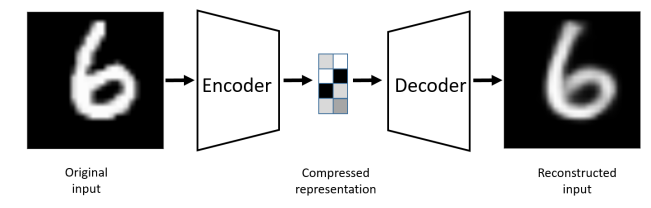
\includegraphics[width=0.5\textwidth]{figures/autoencoder.PNG}
        \caption{Diagram of autoencoders (Source: Bank et. al. 2020)}
        \label{Autoencoder Diagram}
    \end{figure}
    
    \subsection{The VAE Prior Distribution and VampPrior}
    The prior distribution $p(z)$ in the KL divergence term is the unit gaussian $\mathcal{N}(0, I)$ in most VAE implementations. Setting the prior as the unit gaussians has two distinct advantages. First, it is simple to compute a closed-form KL divergence between two gaussians. Second, by choosing a prior distribution with a convex probability density function (PDF), we are less likely to choose points for which the decoder cannot provide quality reconstructions when interpolating between points in the high-density region of the distribution. \\
    
    The unit gaussian is not an ideal prior in minimizing the ELBO; the ideal prior in minimizing the ELBO is the aggregated approximate posterior (\cite{tomczak2018vae}). In practice, this prior would cause overfitting (to say nothing of the computational cost of computing KL divergence with this prior), while on the otherhand, the unit prior would certainly not overfit the embedding model but would likely overreguarlize it (\cite{tomczak2018vae}). As an alternative solution, Tomczak and welling propose the VampPrior, in which the prior is a dynamic mixture of gaussian components. For $K$ learned pseudo-inputs $x_{1},...,x_{K}$, the posterior distribution is given by
    \begin{equation*}
        p_{\gamma}=\frac{1}{K}
        \sum_{k=1}^{K}
        q_{\theta}(z|x_{k})
    \end{equation*}
    where $\lambda$ is the union of the posterior parameters $\theta$ and the additional parameters for learning the pseudo-inputs (\cite{tomczak2018vae}).

    

\end{document}
